\documentclass[11pt]{article}
\usepackage{graphicx}
\usepackage{hyperref}
\usepackage[dvipsnames, svgnames, x11names, hyperref]{xcolor}
\hypersetup{
	colorlinks,
	citecolor=Violet,
	linkcolor=Red,
	urlcolor=Blue}
\usepackage{natbib}
\usepackage{commath, amsmath}
\usepackage{siunitx}
\usepackage{gensymb}

\setlength{\textwidth}{6.5in}
\setlength{\headheight}{0in}
\setlength{\textheight}{8.0in}
\setlength{\hoffset}{0in}
\setlength{\voffset}{0in}
\setlength{\oddsidemargin}{0in}
\setlength{\evensidemargin}{0in}


\title{Homework 9 Solution}

\author{Nana Ama Nyamekye Darpaah}

\begin{document}
	
	\maketitle
	This is my GitHub link: \href{https://github.com/nnd2016/phys-ga2000.git}{Nana Ama's GitHub Link}
	
	\section{Question 1}
	The harmonic and anharmonic oscillator equations are expressed as 
	
\begin{equation}
	\od[2]{x}{t} = -\omega^{2} x
\end{equation}
 and 
\begin{equation}
	\od[2]{x}{t} = -\omega^{2} x^{3}
\end{equation}
	respectively.\\
	
	The fourth-order Runge-Kutta method was employed to solve all the differential equations in this report.
	
	For the harmonic oscillator, the initial conditions of x = 1 and $\od{x}{t}$ had a value of 0, where x represents the amplitude. The initial and final times were $t = 0$ and $t = 50$ respectively. $\omega$ was set equal to 1 in this case. The amplitudes were made to vary at x = 1, 2, and 3 and a plot of position against time was made as shown in \figref{fig:harmonic}. It can be seen that the period has no significant changes as the amplitudes are varied.
	
	\begin{figure}[!h]\begin{center} 
			\vspace{12pt}
			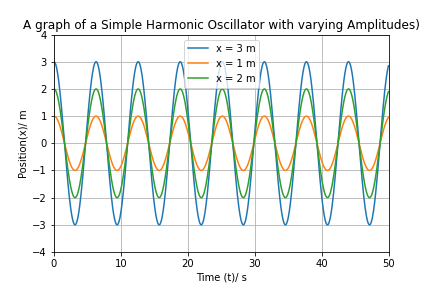
\includegraphics[width=0.7\textwidth]{harmonic.png} 
			\caption{A graph of a simple harmonic oscillator with varying amplitudes }
			\label{fig:harmonic} 
		\end{center}
	\end{figure}

	In the case of the anharmonic oscillator, a plot of time and varying amplitudes was also plotted with the result as shown in \figref{fig:anharmonic1}. The amplitudes were varied with small differences as against that in \figref{fig:anharmonic2}. It can be seen from the 2 plots that the oscillator oscillates faster at higher amplitudes.
	
	\begin{figure}[!h]\begin{center} 
			\vspace{12pt}
			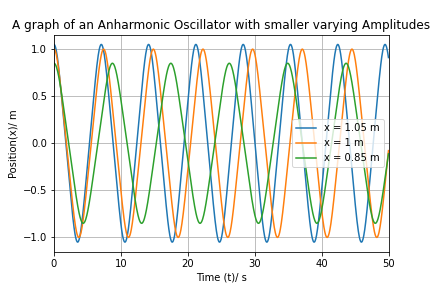
\includegraphics[width=0.7\textwidth]{anharmonic1.png} 
			\caption{A graph of an anharmonic oscillator with small varying amplitudes }
			\label{fig:anharmonic1} 
		\end{center}
	\end{figure}

\begin{figure}[!h]\begin{center} 
		\vspace{12pt}
		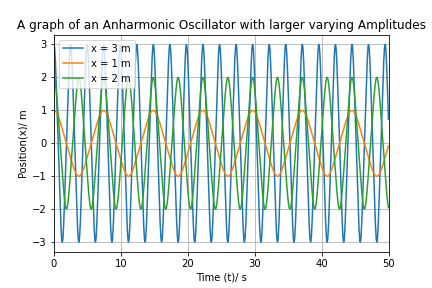
\includegraphics[width=0.7\textwidth]{anharmonic2.png} 
		\caption{A graph of an anharmonic oscillator with large varying amplitudes }
		\label{fig:anharmonic2} 
	\end{center}
\end{figure}

	A phase space plot of velocity against position of the anharmonic oscillator can be seen in \figref{fig:phase_space}.
	\begin{figure}[!h]\begin{center} 
			\vspace{12pt}
			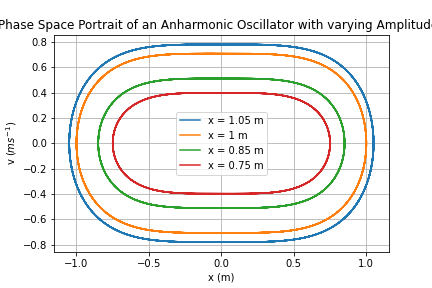
\includegraphics[width=0.7\textwidth]{phase_space.png} 
			\caption{Phase Space plot of an anharmonic oscillator at varying amplitudes }
			\label{fig:phase_space} 
		\end{center}
	\end{figure}
\\
	The equation of the Van der Pol oscillator is given by
	
	\begin{equation}
		\od[2]{x}{t} = \mu (1-x^{2})\od{x}{t} - \omega^{2} x
	\end{equation}



	The constant $\mu$ was made to vary as $\mu = 1, 2, 4$ and the phase space diagrams to each value of mu were plotted on the same graph as shown in \figref{fig:vanderpol}. Here, the initial and final times were given as $t=0$ and $t=20$ respectively and $h$ was made small enough to ensure the smoothness of the plot. 
	\begin{figure}[!h]\begin{center} 
			\vspace{12pt}
			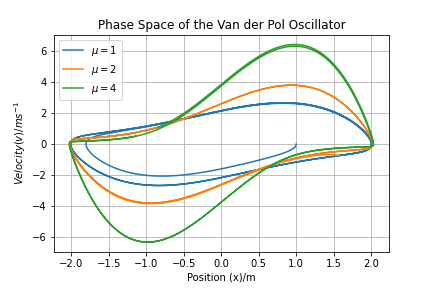
\includegraphics[width=0.7\textwidth]{vanderpol.png} 
			\caption{Phase Space plot of a Van der Pol oscillator at varying amplitudes }
			\label{fig:vanderpol} 
		\end{center}
	\end{figure}
	
	




\section{Question 2}
Air resistance is expressed as 
\begin{equation}
	F = \frac{1}{2} \pi R^{2} \rho C v^2
\end{equation}
where R is the radius of the spherical cannonball , $\rho$ is the density of air, $C$ is the drag coefficient and $v$ is the velocity, $v = \sqrt{\dot{x}^2 + \dot{y}^2}$.

The total forces acting on the cannonball are expressed as
\begin{equation}
	F = ma = F_{grav} + F_{drag}
\end{equation}
where $a$ is the acceleration, $F_{grav}$ is the gravitational force and $F_{drag}$ is the air resistance force. This implies
\begin{equation}
	\ddot{r} = -mg \hat{y} - \frac{1}{2}\pi R^{2}\rho C v^{2} \hat{v}
\end{equation}
and $\hat{v} = \frac{\vec{v}}{\left | \vec{v} \right |}$ \\

For the x-direction,


\begin{align}
		m\ddot{x} & = -\frac{1}{2} \pi R^{2} \rho C v^2 \frac{\dot{x}}{v} \\
	& = -\frac{1}{2} \pi R^{2} \rho C \dot{x} \sqrt{\dot{x}^{2} + \dot{y}^{2}}
\end{align}
 
 Likewise, for the y-direction,
 \begin{align}
 	m\ddot{y} & = -mg -\frac{1}{2} \pi R^{2} \rho C v^2 \frac{\dot{y}}{v} \\
 	& = -g -\frac{1}{2} \pi R^{2} \rho C \dot{y} \sqrt{\dot{x}^{2} + \dot{y}^{2}}
 \end{align}
Hence, the 2 differential equations are

\begin{align}
	\ddot{x} & = -\frac{1}{2} \pi R^{2} \rho C \dot{x} \sqrt{\dot{x}^{2} + \dot{y}^{2}}\\
	\ddot{y} & = -g -\frac{1}{2} \pi R^{2} \rho C \dot{y} \sqrt{\dot{x}^{2} + \dot{y}^{2}}
\end{align}


Rescaling the variables to produce a unitless equation was made through the $t = t'/T$ subsitution as well as the $x = gT^{2} x'$ and $y = gT^{2} y'$ .  


 \begin{figure}[!h]\begin{center} 
 		\vspace{12pt}
 		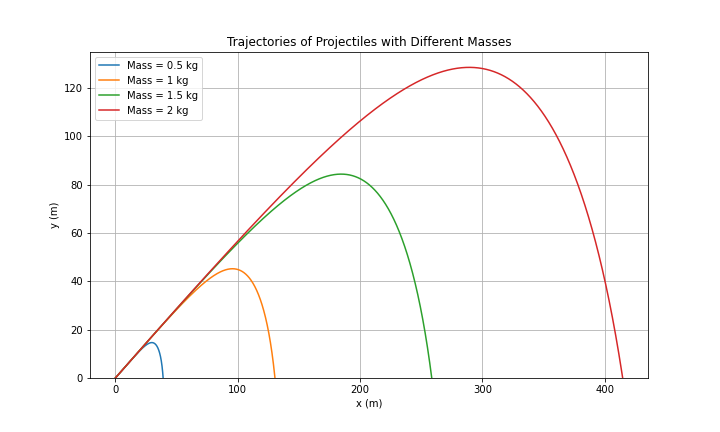
\includegraphics[width=0.8\textwidth]{projectiles.png} 
 		\caption{Trajectories of Projectile Motion with Air Resistance at varying Masses}
 		\label{fig:projectile} 
 	\end{center}
 \end{figure}
 A series of trajectories for different masses of the cannonball was plotted with the initial velocity being $100 ms^{-1}$ at $30\degree$ to the horizontal as shown in \figref{fig:projectile}. As shown, the total horizontal distance does indeed depend on the mass of the projectile. From the plot, it is seen that heavier masses travel further than lighter masses.



\end{document}